\begin{frame}
    \titlepage
\end{frame}

\begin{frame}{What's that?}
    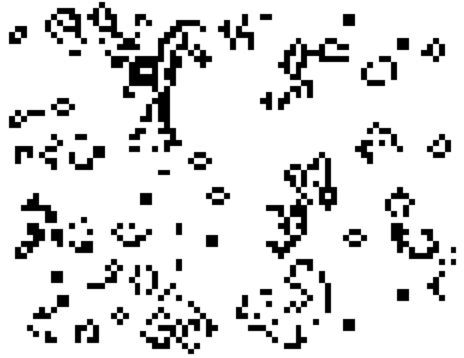
\includegraphics[width=0.9\linewidth]{../paper/figures/game_of_life_still}
\end{frame}

\begin{frame}{Overview}
    \begin{columns}
        \column{0.333\linewidth}
        \begin{figure}
            \centering
            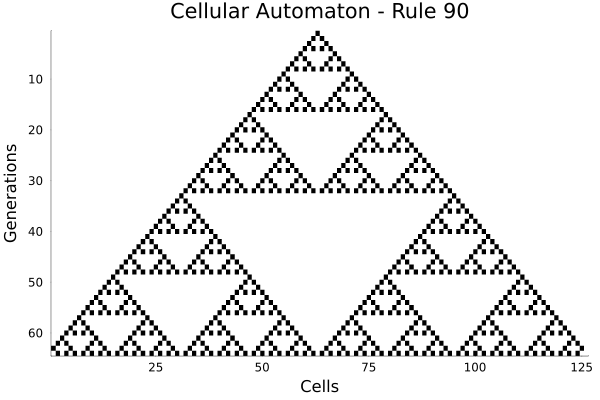
\includegraphics[width=0.8\textwidth]{../paper/figures/rule90}
            \caption{1D Cellular Automata}
        \end{figure}
        \column{0.333\linewidth}
        \begin{figure}
            \centering
            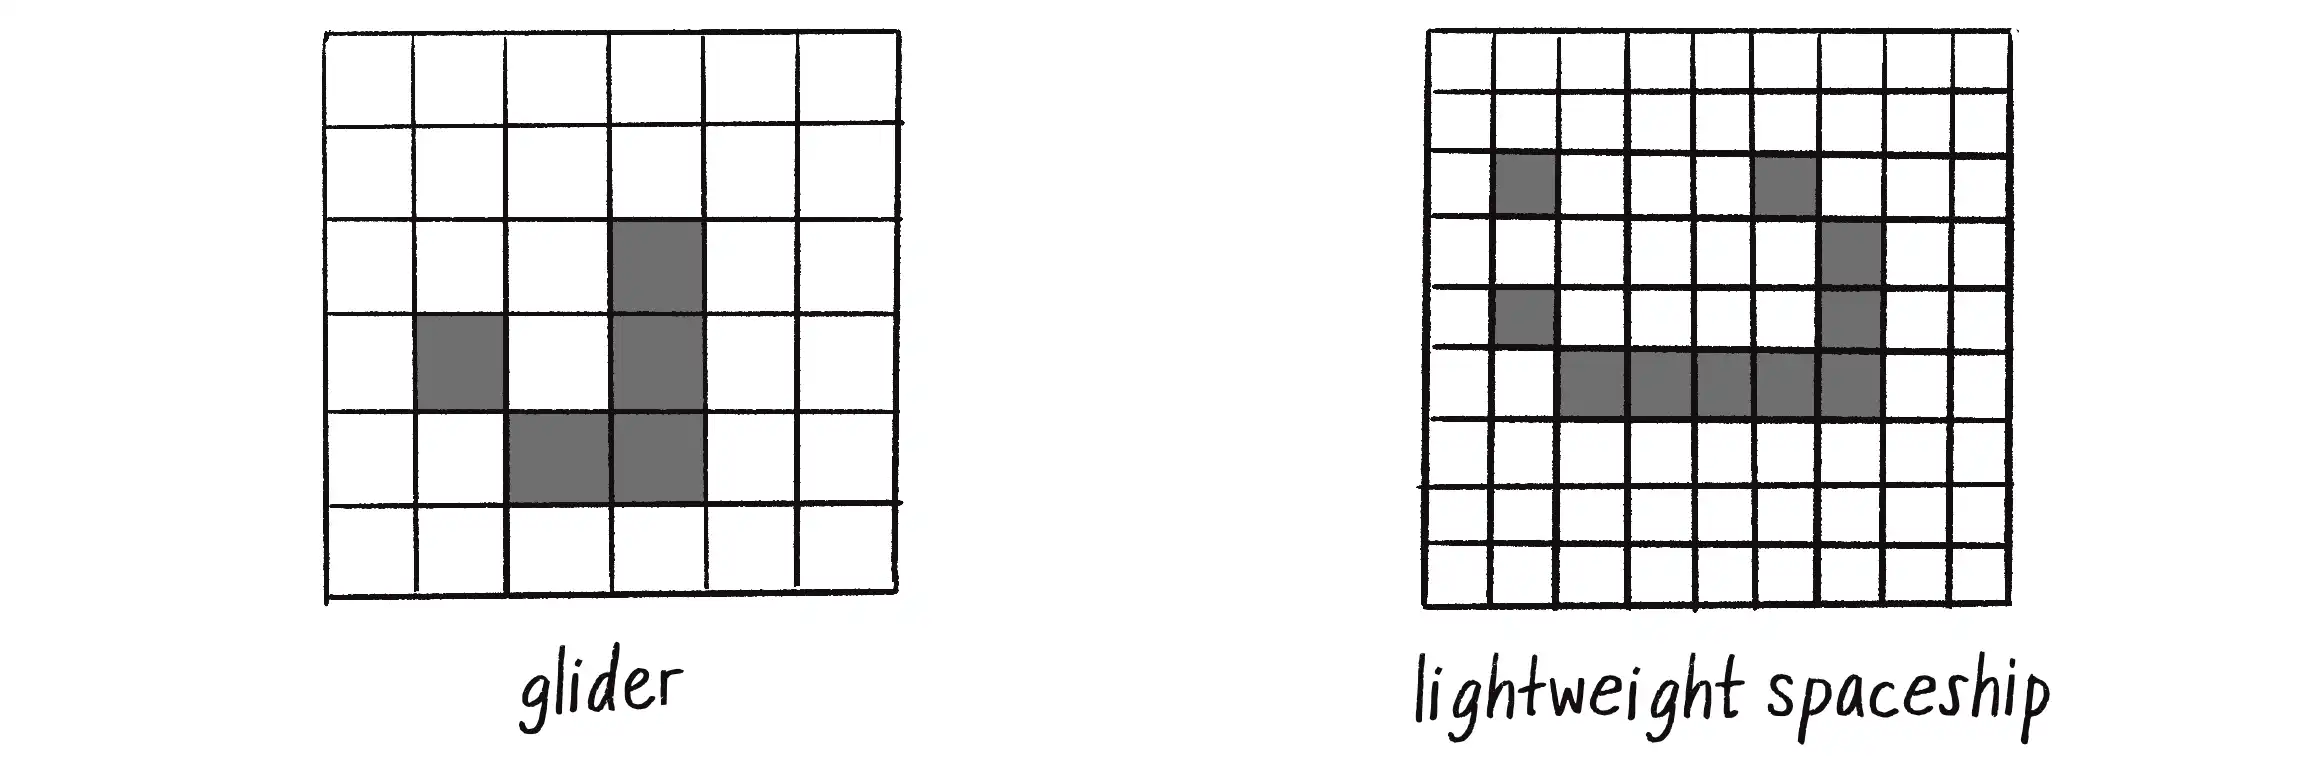
\includegraphics[width=0.8\textwidth]{../paper/figures/spaceship}
            \caption{2D Cellular Automata}
        \end{figure}
        \column{0.333\linewidth}
        \begin{figure}
            \centering
            
\includegraphics[width=0.8\textwidth]{../paper/figures/julia}
            \caption{Julia Implementation\footnotemark}
        \end{figure}
    \end{columns}
    \footnotetext[1]{\url{https://commons.wikimedia.org/wiki/File:Julia_Programming_Language_Logo.svg}}
\end{frame}


\section{Introduction}
\begin{frame}{What are Cellular Automata?}
    \begin{itemize}
        \item Discrete models: grid of cells, each with a state
        \item Simple, local rules $\rightarrow$ complex global behavior
        \item Used for simulating complex systems (urban, physics, biology)
        \item Example: Conway's Game of Life
    \end{itemize}
\end{frame}


\section{1D Cellular Automata}
\begin{frame}{1D Cellular Automata: Theory}
    \begin{itemize}
        \item Cells in a 1D array, each with a state (e.g., 0 or 1)
        \item Neighborhood: e.g. cell itself + left/right neighbors
        \item Update rules: Neighborhood $\rightarrow$ next state
    \end{itemize}
\end{frame}

\begin{frame}{1D CA: Ruleset}
    \begin{figure}
        \centering
        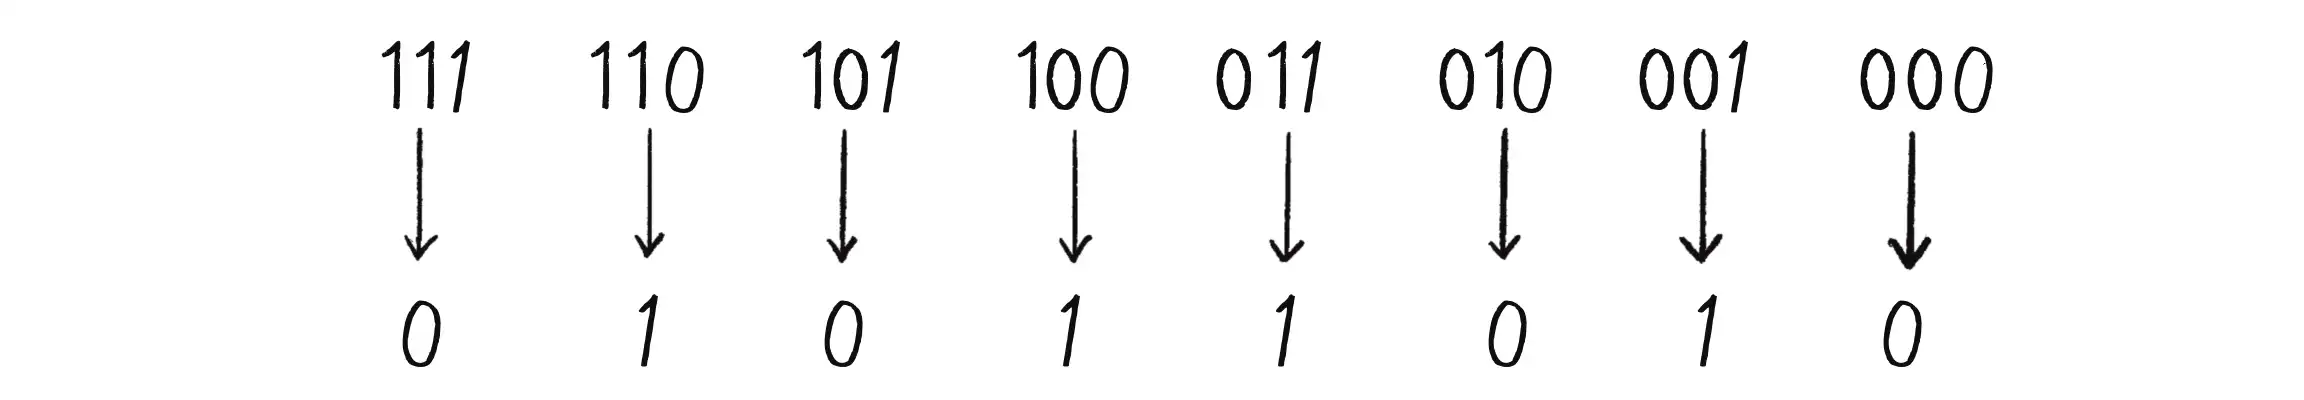
\includegraphics[width=\textwidth]{../paper/figures/ruleset_example.png}
        \caption{Example: Mapping neighborhood to next state (here rule number 90)}
    \end{figure}
\end{frame}

\begin{frame}{1D CA: Visualization}
    \begin{figure}
        \centering
        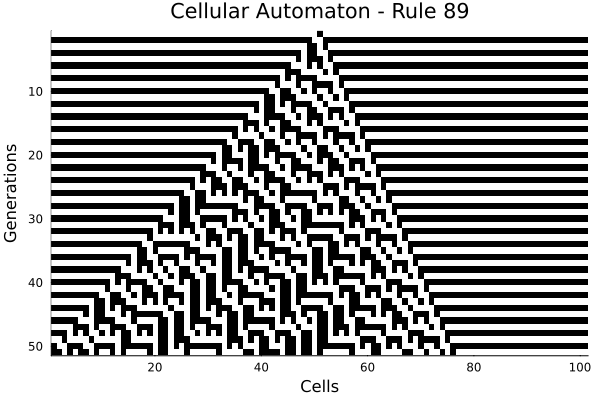
\includegraphics[width=0.5\textwidth]{../paper/figures/carule89}
        \caption{Visualization of generations as rows in a 2D grid}

    \end{figure}

\end{frame}


\begin{frame}{Wolfram Classification}
    \begin{columns}
        \column{0.4\linewidth}
        \begin{itemize}
            \item \textbf{Class 1:} Uniformity (stable)
            \item \textbf{Class 2:} Repetition (periodic)
            \item \textbf{Class 3:} Random (chaotic)
            \item \textbf{Class 4:} Complexity (mix of order/chaos)
        \end{itemize}
        \column{0.6\linewidth}
        \begin{figure}
            \centering
            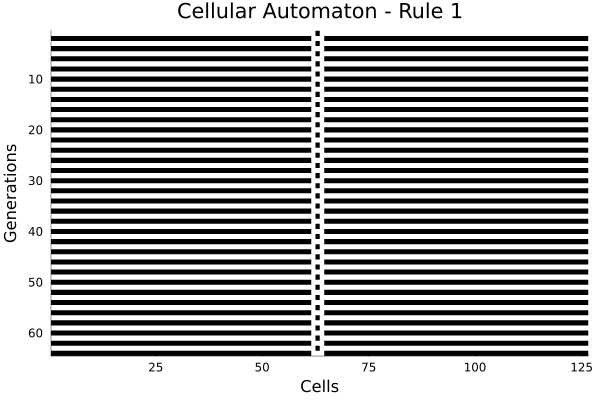
\includegraphics[width=0.8\textwidth]{../paper/figures/rule1.png}
            \caption{Rule 1: An example of Class 2 (repetitive)}
        \end{figure}
    \end{columns}
\end{frame}


\section{2D Cellular Automata}
\begin{frame}{2D Cellular Automata: Game of Life}
    \begin{columns}
        \column{0.4\linewidth}
        \begin{itemize}
            \item Grid of cells, each with $8$ neighbors
            \item \textbf{Rules:}
                  \begin{itemize}
                      \item Birth: exactly $3$ alive neighbors
                      \item Survival: $2$ or $3$ alive neighbors
                      \item Death: $<2$ or $>3$ alive neighbors
                  \end{itemize}
        \end{itemize}
        \column{0.6\linewidth}
        \begin{figure}
            \centering
            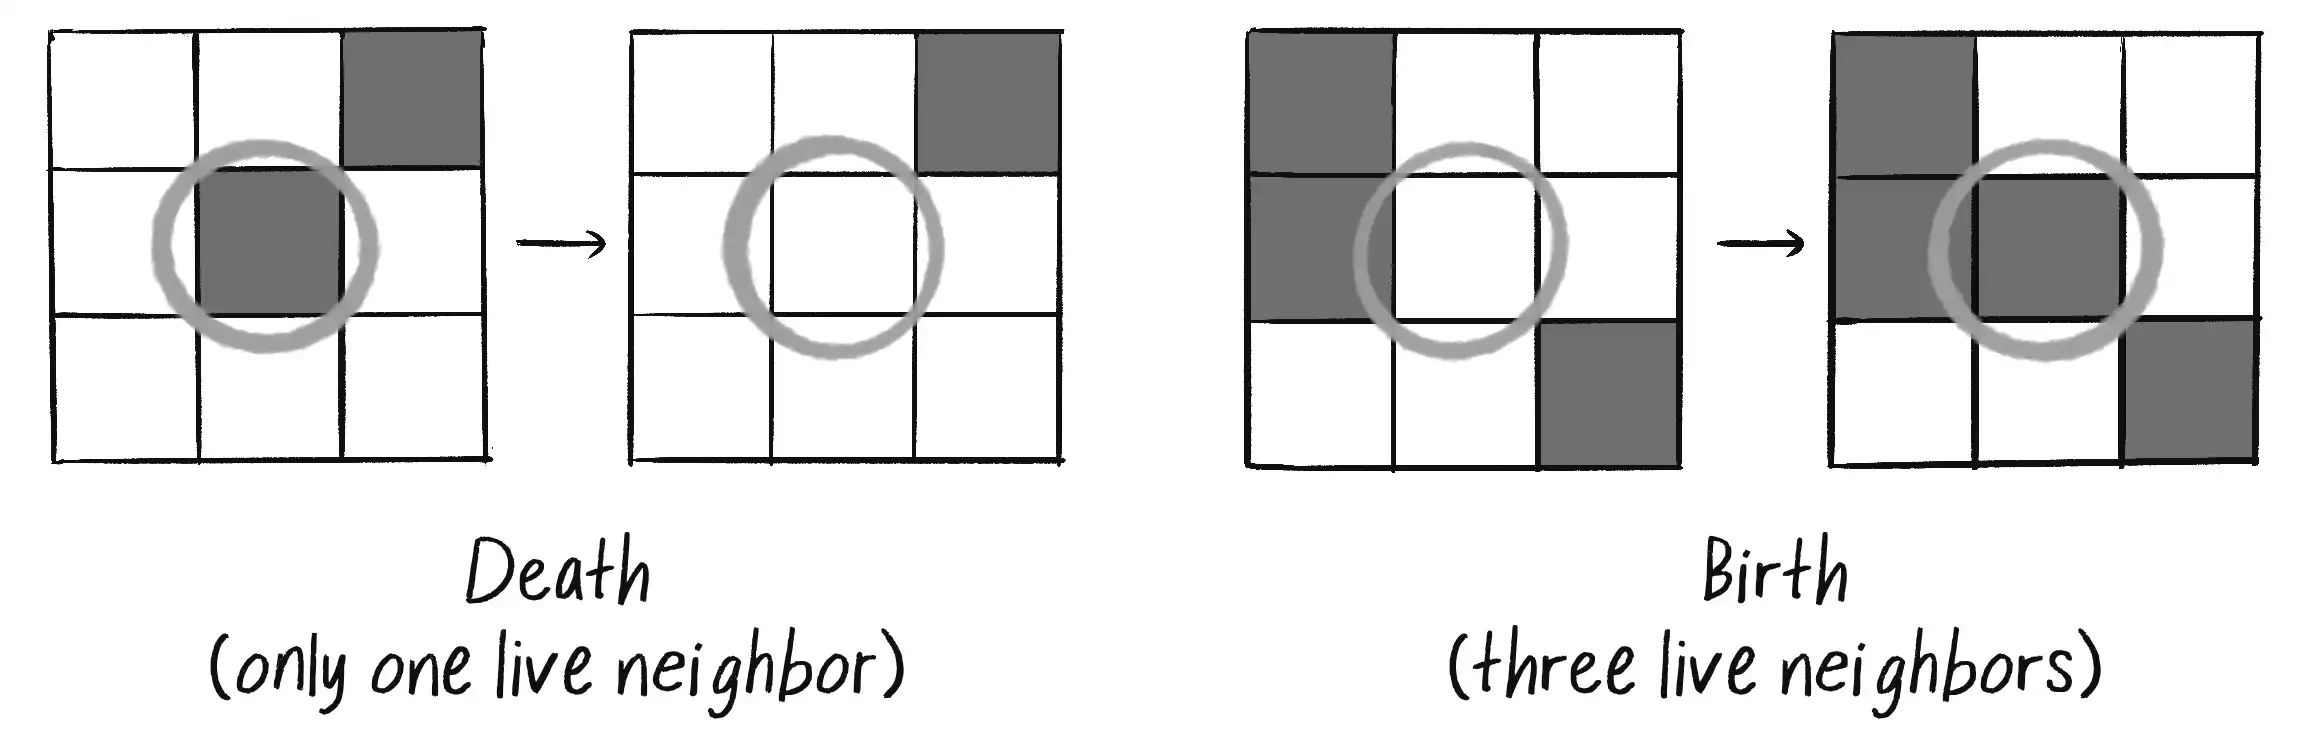
\includegraphics[width=\textwidth]{../paper/figures/game_of_life_examples}
            \caption{Examples of scenarios in the Game of Life\footnotemark}
        \end{figure}
    \end{columns}
    \footnotetext[2]{\url{https://natureofcode.com/static/99dd5b32b72ce094d5a77f749c2ab9f0/3ca65/07_ca_28.webp}}
\end{frame}

\begin{frame}{Game of Life: Patterns}
    \begin{columns}
        \column{0.4\linewidth}
        \begin{itemize}
            \item \textbf{Stable:} Do not change
            \item \textbf{Oscillators:} Repeat after $n$ steps
            \item \textbf{Spaceships:} Move across grid
            \item \textbf{Guns:} Emit other patterns
        \end{itemize}
        \column{0.6\linewidth}
        \centering
        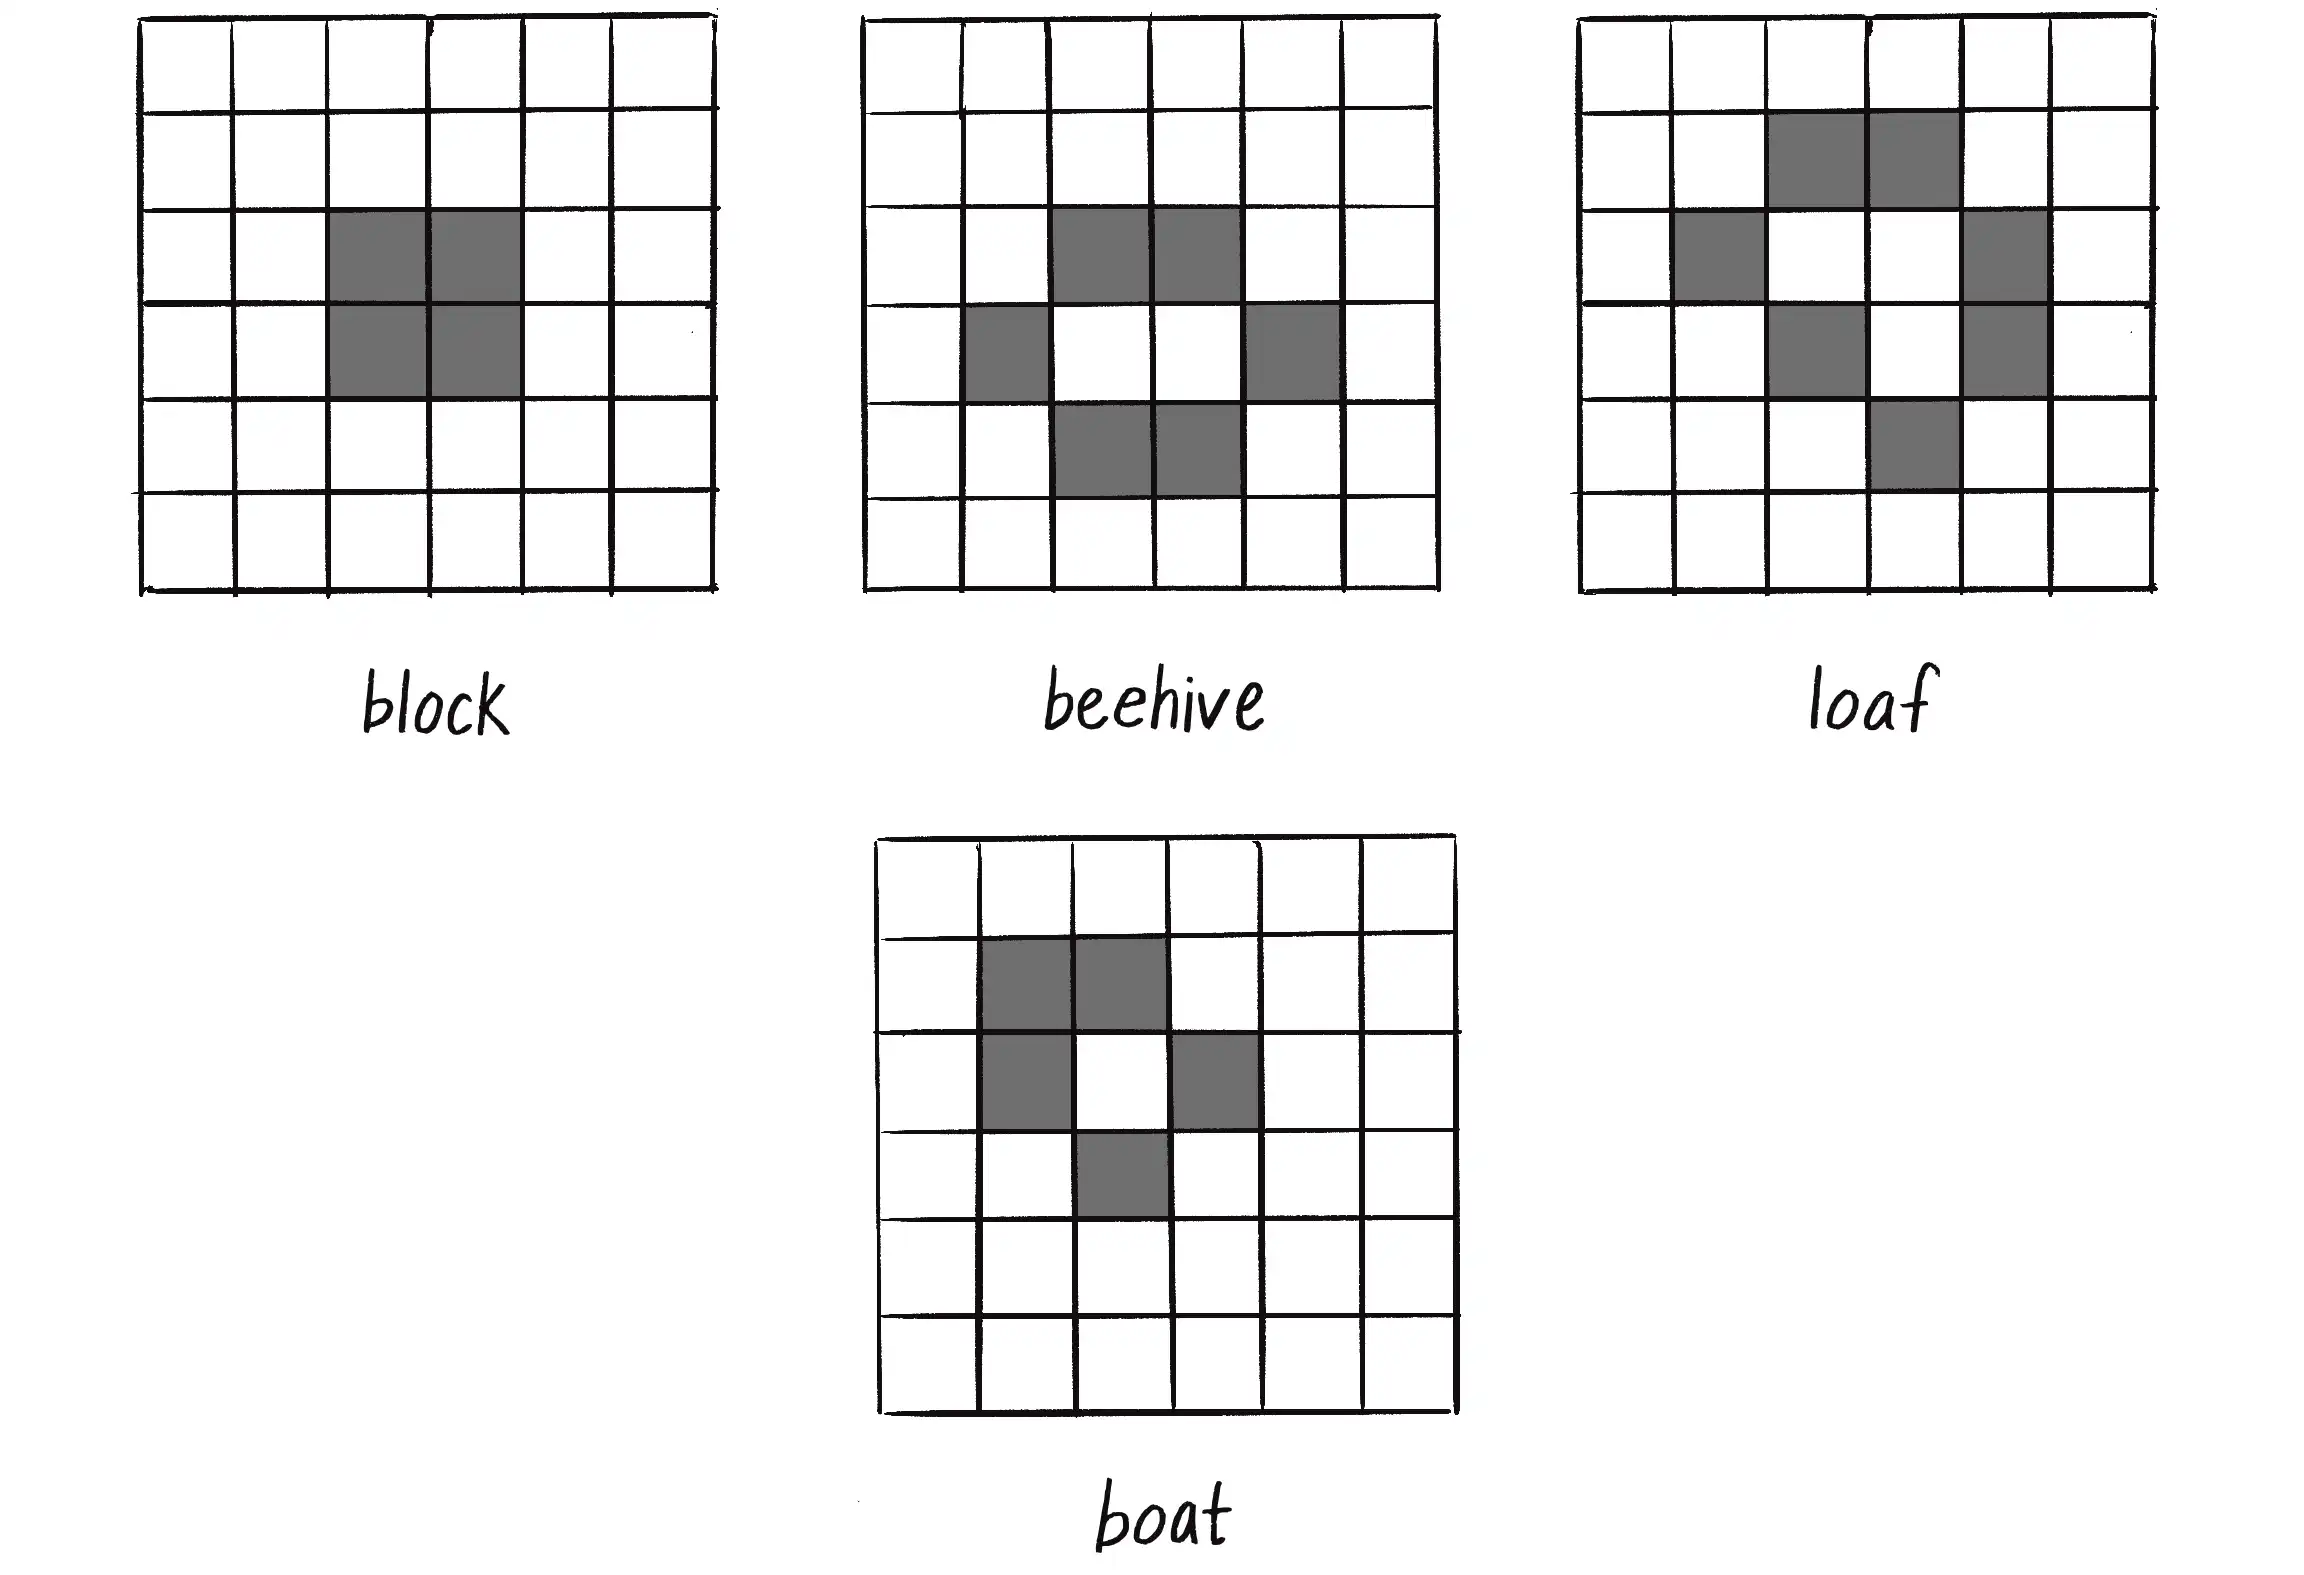
\includegraphics[height=8em]{../paper/figures/stable}\\
        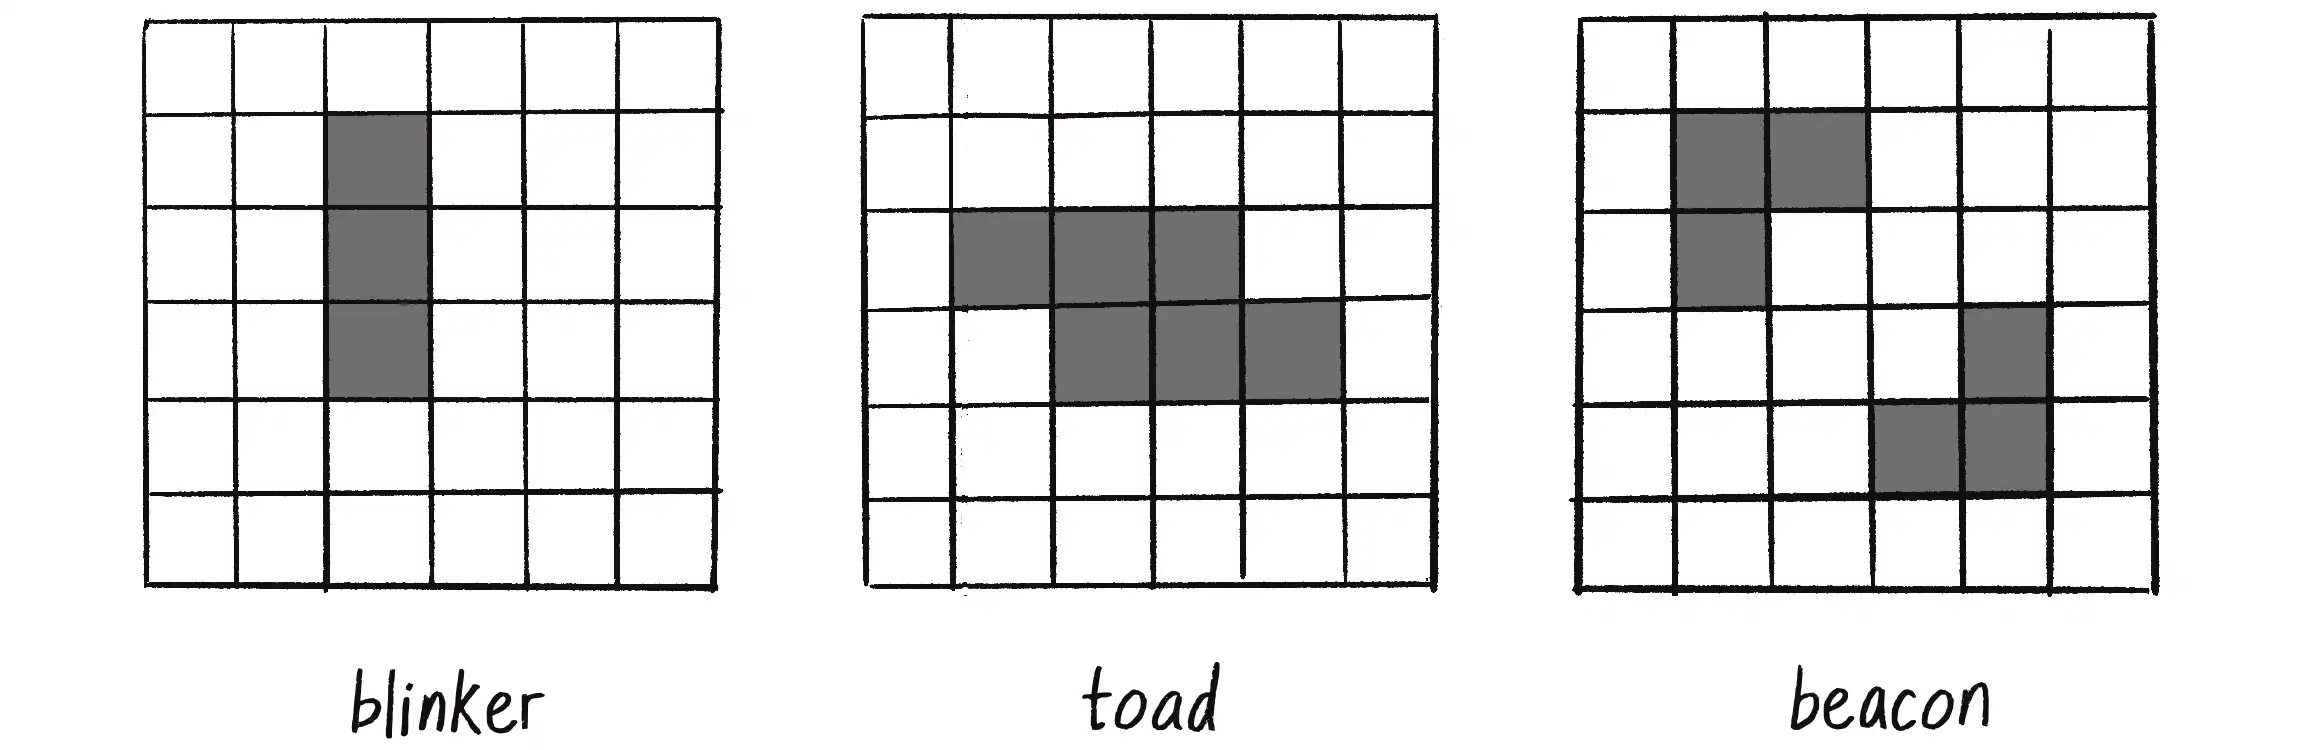
\includegraphics[height=5em]{../paper/figures/oscillator}\\
        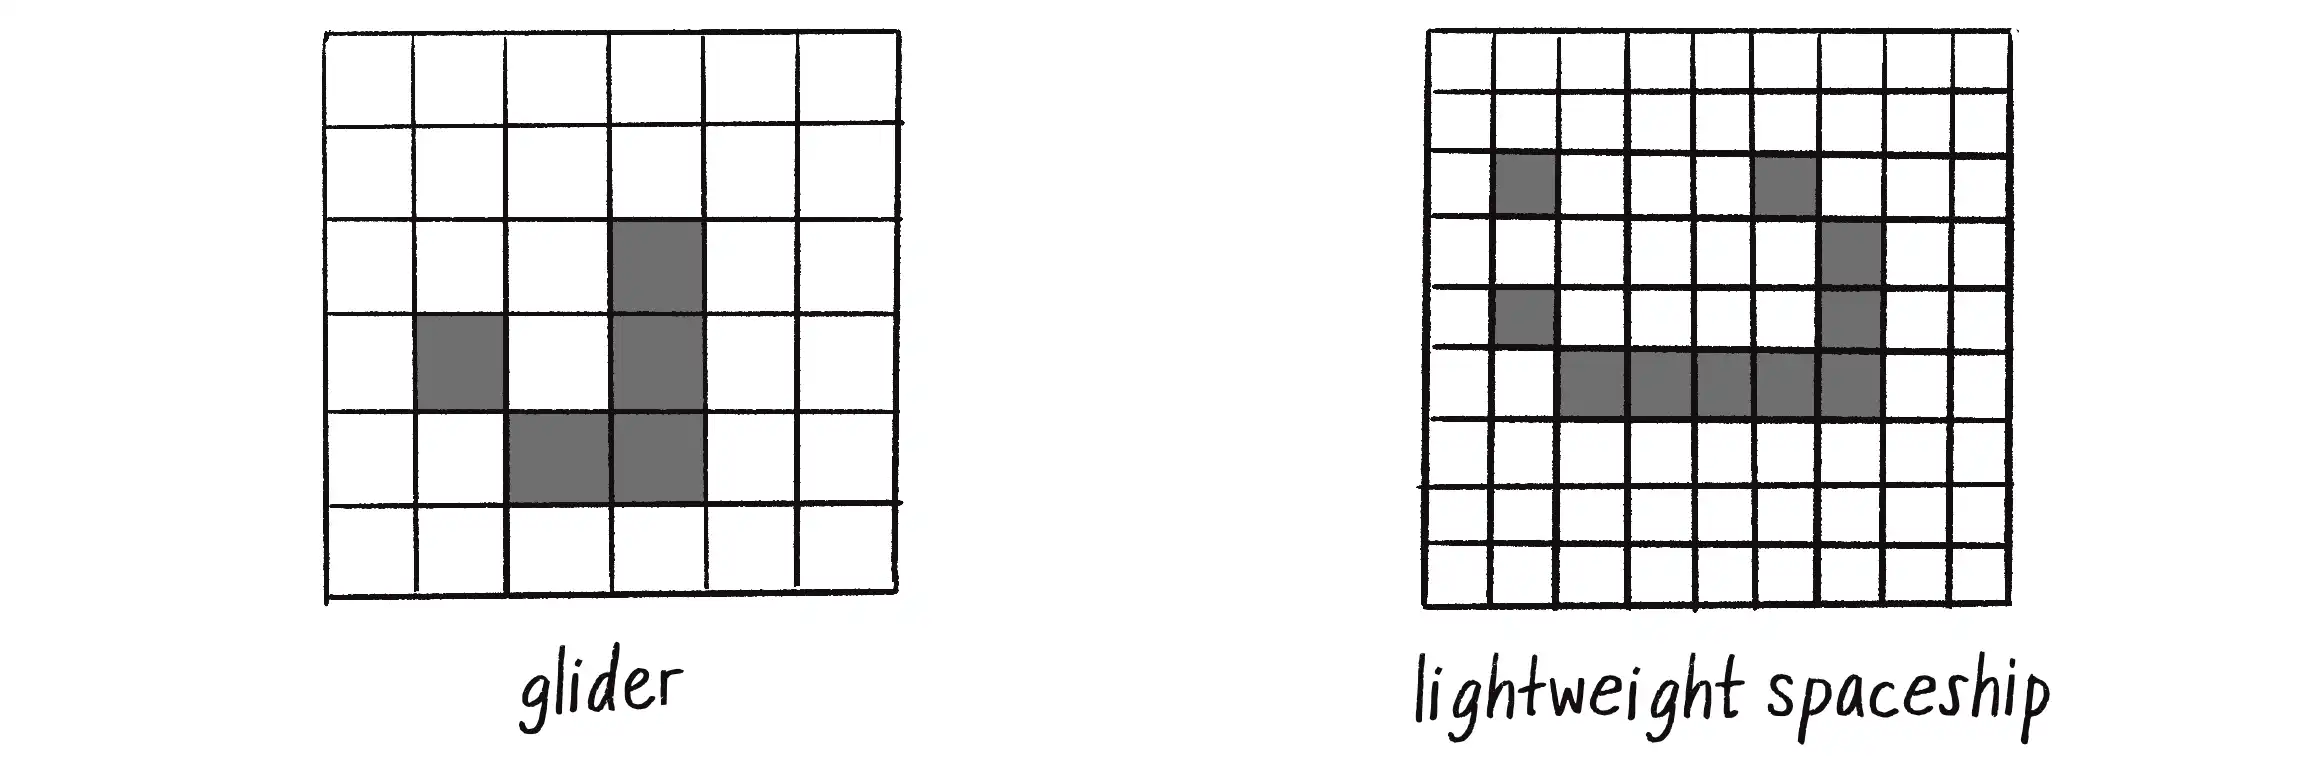
\includegraphics[height=5em]{../paper/figures/spaceship}

    \end{columns}
\end{frame}


\section{Julia}
\begin{frame}[fragile]{1D CA in Julia - apply\_rule function}
    \begin{figure}
        \centering
        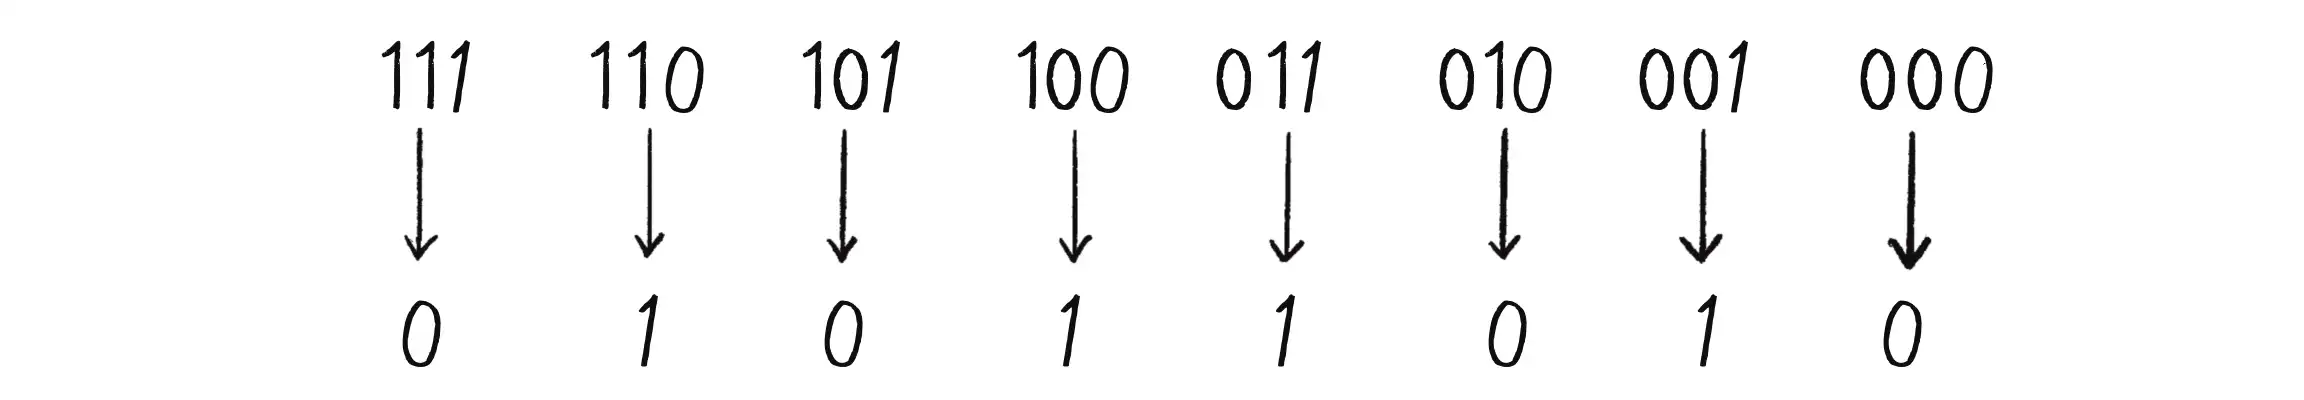
\includegraphics[width=\textwidth]{../paper/figures/ruleset_example.png}
        \caption{Example: Mapping neighborhood to next state (here rule number 90)}
    \end{figure}
    \begin{lstlisting}[language=Julia, caption={apply\_rule function for 1D CA}, basicstyle=\ttfamily\scriptsize]
function apply_rule(left::Int, center::Int, right::Int, rule_number::Int)::Int
    neighborhood_value = left * 4 + center * 2 + right * 1
    return (rule_number >> neighborhood_value) & 1
end
\end{lstlisting}
\end{frame}

\begin{frame}{Rest of 1D CA Implementation}
    \begin{itemize}
        \item \textbf{Initialization:} Create initial state (e.g., random)
        \item \textbf{Update:} Apply rules to each cell
        \item \textbf{Visualization:} Display generations as rows in a 2D grid
    \end{itemize}
\end{frame}

\begin{frame}{Game of Life in Julia}
    \begin{itemize}
        \item \textbf{Initialization:} Create intial state (e.g., random)
        \item \textbf{Update:} Apply Game of Life rules to each cell
        \item \textbf{Visualization:} Display grid as a row of 2D images or a GIF
    \end{itemize}

\end{frame}

\begin{frame}{Extending Game of Life: Infection Simulation}
    \begin{itemize}
        \item \textbf{Infection Model:} Cells can be healthy, infected, dead/not existing
        \item \textbf{Rules:}
              \begin{itemize}
                  \item Infected cells infect neighbors
                  \item Infected cells can die
                  \item Healthy cells can reproduce
              \end{itemize}
        \item \textbf{Visualization:} Display grid with different colors for each state
    \end{itemize}

\end{frame}


\begin{frame}{Why Julia for Simulation?}
    \begin{itemize}
        \item \textbf{Performance:} Fast, optimized for numerical computing
        \item \textbf{Syntax:} Concise, math-like, less verbose than JavaScript
        \item \textbf{Ecosystem:} Rich packages for simulation and visualization
    \end{itemize}
\end{frame}


\section{Discussion}
\begin{frame}{Discussion}
    \begin{itemize}
        \item Cellular automata are used in simulations like Lattice Boltzmann for fluid dynamics.
        \item LBM is efficient and parallelizable due to local interactions.
        \item PDEs simulate continuous systems but need complex numerical methods.
        \item Cellular automata use simple, discrete rules; not direct PDE replacements.
        \item Time steps and update rules are common in many simulation methods.
    \end{itemize}

\end{frame}


\section{Conclusions}
\begin{frame}{Conclusions / Relation to seminar}
    \begin{itemize}
        \item Covered cellular automata basics, especially Game of Life.
        \item Showed Julia implementation and visualization.
        \item Simple rules yield complex behavior.
        \item Julia is fast and flexible for simulations.
        \item Cellular automata help study emergent phenomena.
    \end{itemize}
\end{frame}


\begin{frame}{Thanks}
    \centering
    \Huge
    Thank you for your attention!
\end{frame}
